\documentclass[tikz,border=3mm]{standalone}
\usepackage{amsmath}
\begin{document}
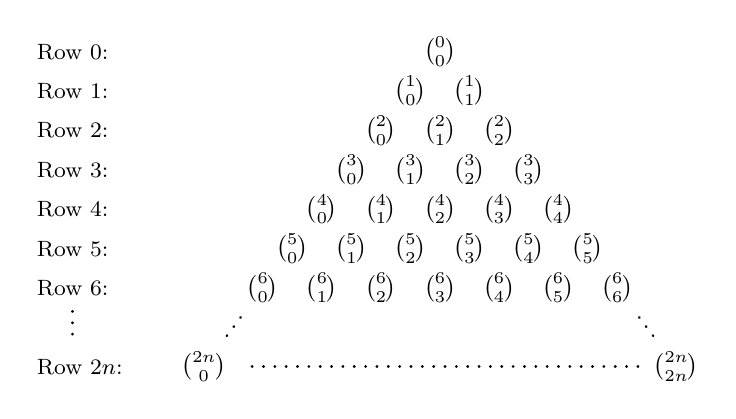
\begin{tikzpicture}[x=0.75cm,y=0.5cm, 
  pascal node/.style={font=\footnotesize}, 
  row node/.style={font=\footnotesize, anchor=west, shift=(180:1)},
  Dotted/.style={% https://tex.stackexchange.com/a/52856/194703
  dash pattern=on 0.1\pgflinewidth off #1\pgflinewidth,line cap=round,
  shorten >=2pt,shorten <=2pt,line width=1pt},
  Dotted/.default=4,thick]
  \def\NPascal{6}
  \def\offset{2}
  \draw  
    foreach \n in {0,...,\NPascal} { 
      (-\NPascal/2-1-\offset, -\n) node (rn-\n) [row node/.try]{Row \n:}
        \foreach \k in {0,...,\n}{
          (-\n/2+\k,-\n) node (pn-\n-\k) [pascal node/.try] {%
             $\binom{\n}{\k}$  
        }}}
    (-\NPascal/2-1-\offset, -\NPascal-2) node (rn-N) [row node/.try]{Row $2n$:}
    (-\NPascal/2-1, -\NPascal-2) node (pn-N-0) [pascal node/.try] {$\binom{2n}{0}$}
    (\NPascal/2+1, -\NPascal-2) node (pn-N-N) [pascal node/.try] {$\binom{2n}{2n}$}
    (rn-\NPascal) edge[Dotted] (rn-N.north-|rn-\NPascal)
    (pn-\NPascal-0) edge[Dotted] (pn-N-0) 
    (pn-\NPascal-\NPascal) edge[Dotted] (pn-N-N)
    (pn-N-N) edge[Dotted] (pn-N-0);
\end{tikzpicture}       
\end{document}